\chapter{Visual conventions}

This chapter will address the visual convention connected to population projection. 
Within the field of spatial convention there are multiple convention, however not all of these are relevant in this particular context. To understand which conventions are relevant for visualizing data one must understand the properties of the data to be visualized. Spatial data can be presented as either discrete-objects or continuous-fields also known as vector and raster data. \citep{objectsNFields} These two types of data have different ways of being visualised. 
As mentioned in chapter \ref{Add chapter} the data is in the raster format and is sequential. Visual conventions connected to discrete-objects will therefore not be covered.

Visual conventions connected to raster maps are largely covered by convention connected to color. 
\subsection{Color}
A color can be defined by three parameters: hue, saturation and lightness. These different concept have all been illustrated in figure \ref{MunsellColorSystem}.

\begin{figure} [H]
	\centering
	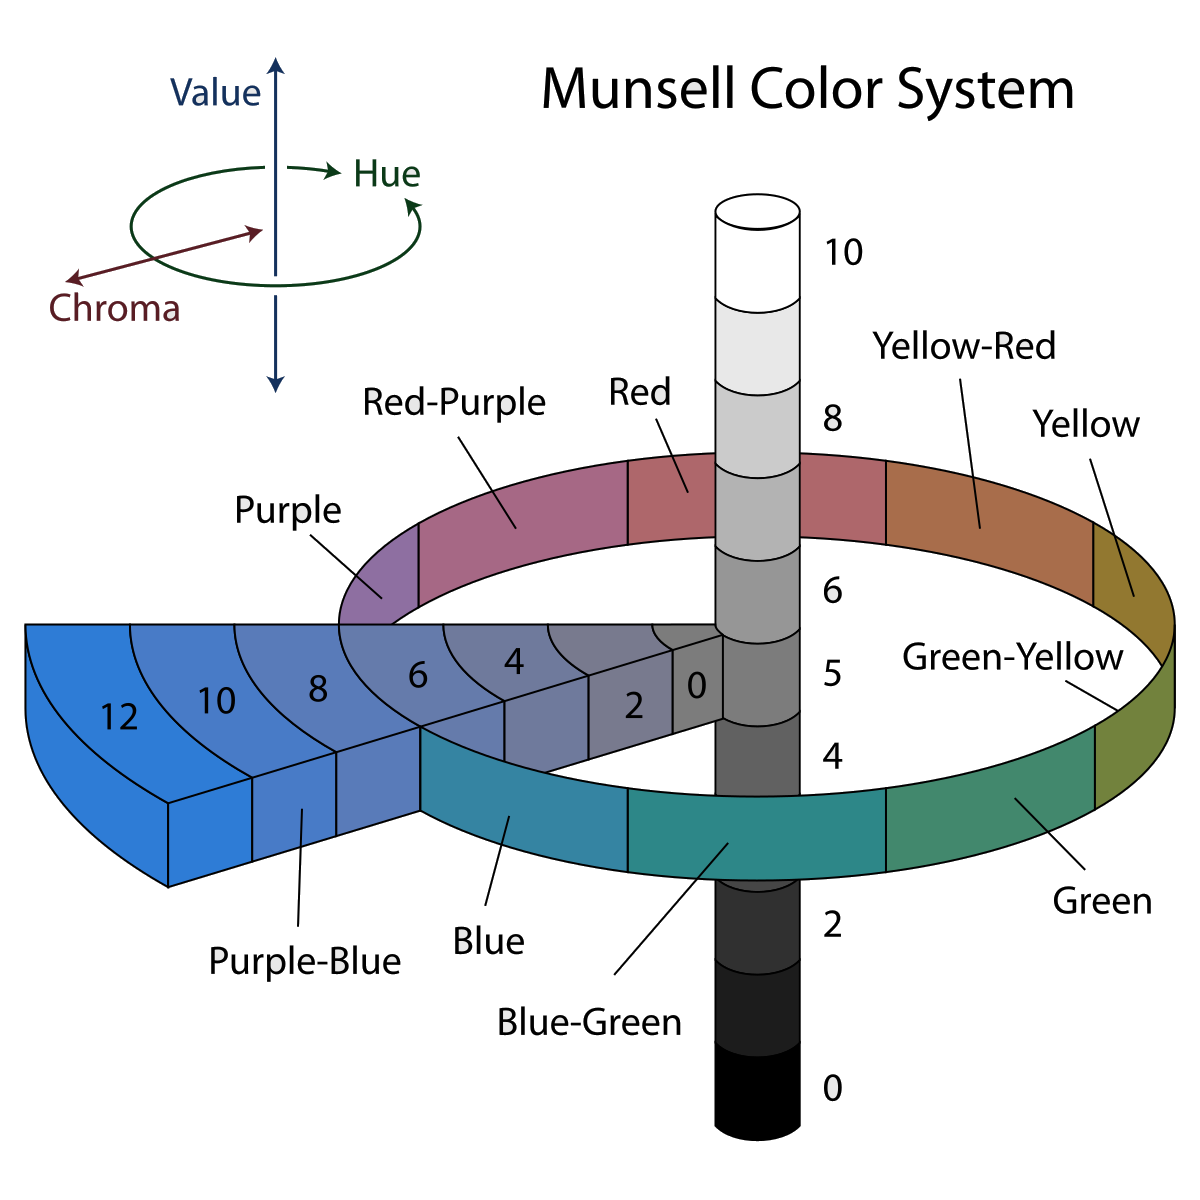
\includegraphics[width=.8\textwidth]{Pictures/MunsellColorSystem}
	\caption{Illustration of the concepts: hue, saturation and lightness. Source: \citet{JacobRus}}
	\label{MunsellColorSystem}
\end{figure}

\textbf{Hue}

The hue is what would traditionally be referred to as colors (red, green, yellow). In the figure the hue is illustrated as the circle around the column.

\textbf{Saturation}

The saturation is also referred to by some authors as chroma, intensity or purity. It is a measurement for how vivid the color is. A color with a low saturation would be close to the color grey. If the saturation increases more of the color pigment is added to the color, until there is no trace of grey left. The saturation has a value from 100\% (fully colored) to 0\% (grey). It is illustrated in the figure as the distance from the center.

\textbf{Lightness}

A measurement of the color’s lightness or darkness. In the literature this is often referred to as the colors value, but Brewer remarks that this use of terminology is not ideal in data science since "value" also could refer to the data values. It is illustrated as the vertical axis in the figure.  \citep{Dent}

 
\subsubsection{Selecting a color scheme}
There are multiple elements, that should be considered, when choosing a color scheme.
Naturally the different colors should be easily distinguishable, but one should also consider the user of the map and the medium used for presenting the map. The right choice of color pattern allows the user to see patterns in complex data, which otherwise would be obscured. 


Cindy Brewer divides color schemes into the four categories; binary, qualitative, diverging and sequential. These categories and combinations between them have been visualized in figure \ref{BrewerDataTypes}. \citep{Brewer94}

\begin{figure} [H]
	\centering
	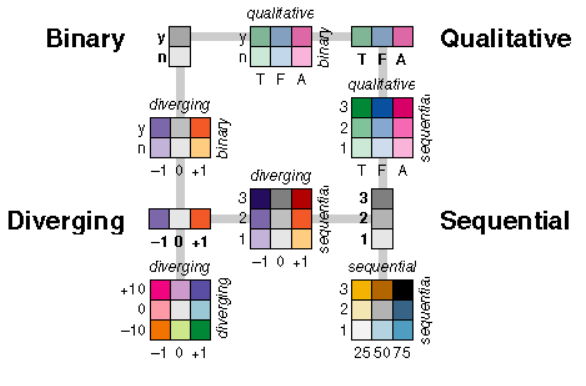
\includegraphics[width=.8\textwidth]{Pictures/BrewerDataTypes}
	\caption{Illustration of the different categories of color schemes. Source: \citet{ColorGuidelines}}
	\label{BrewerDataTypes}
\end{figure}
 

Each of these categories are good for visualizing different kinds of data. The qualitative is well suited for illustrating nominal data. This color scheme is for instance commonly used for land use maps. The binary scheme is a qualitative scheme, but with only two categories. A example of a use case for this scheme could be visualizing whether countries are members of the European Union or not. 
The sequential scheme is useful for illustrating the ordered data going from low values to higher ones. An example of this could be height of vegetation. The differentiation between the values are illustrated with differences in lightness.
The diverging scheme is similar to having two sequential color schemes. This enables highlighting a critical value in the middle of the data. It is for example being used to illustrate temperatures, where the neutral middle value would be 0$^o$C. \citep{Brewer94}


Based on these categories of color schemes Brewer have developed an online tool, colorbrewer2.org, which can aid mapmakers in picking a color scheme. This tool also takes into colorblindness into consideration and inform the user if a colorscheme is suitable for printing or viewing on small screens. \citep{ColorBrewer}



\subsubsection{Visual conventions for colors}
The conventions can be divided based on whether the visualized data is qualitative or quantitative. The qualitative datasets have many historical convention – like using green colors for vegetation or using blue for water. 
It is not the same case for quantitative data, where “No conventions exist for color choice on quantitative maps. (for example, population density maps are always blue, income maps are always green, and so on)” \citep{Dent}. There are however convention for the choice of lightness, where "light is less - dark is more"
% http://www.geo.uzh.ch/~sara/pubs/garlandini_fabs09.pdf

\citep{LightIsLess} %Page1






%
%
%
%\chapter{Initial research and related work}
%
%Prior to developing the tool some initial experimentation with the case dataset was conducted. This lead to some core concepts which should apply to the developed tool. After this existing tool is described, which follows many of these core concepts.
















